\documentclass{beamer}
\usepackage{array}
\usepackage{graphicx}
\usepackage{german}
%\usepackage{txfonts}

\mode<beamer>{%
\usetheme[hideothersubsections,hidetitle]{Hannover}
}
\title[]{Partielle Differentialgleichungen}
\subtitle{2. Sitzung}
\date[2.~M"arz 2016]{2.~M"arz 2016}
\author{Prof.~Dr.~Andreas M"uller}
\begin{document}

\begin{frame}
\titlepage
\end{frame}

\begin{frame}
\frametitle{Geometrie}
\begin{center}
\includegraphics[width=\hsize]{../../skript/images/ode-1.pdf}
\end{center}
\[
y'=\frac16y+e^{-\frac{x}6}\cos x
\qquad\Leftrightarrow\qquad
e^{-\frac{x}6}\cos x
+
\frac16y
-
y'
=0
\]
\end{frame}

\begin{frame}
\frametitle{Plan}
\begin{enumerate}
\item Kurve
\pause
$\to$ Fl"ache
\[
y = f(x)
\qquad\to \qquad
z = u(x,y)
\]
\pause
\item Steigung
\pause
$\to$ zwei Ableitungen
$\displaystyle\frac{\partial u}{\partial x}$,
$\displaystyle\frac{\partial u}{\partial y}$
\[
F(x,y,y')=0
\qquad\to \qquad
F\biggl(x,y,u,\frac{\partial u}{\partial x},\frac{\partial u}{\partial y}
\biggr)=0
\]
\pause
{\bf Wichtig:} Nicht Tangentialebene!
\pause
\item Anfangswerte
\pause
$\to$ Cauchy-Problem
\[
y(0)=y_0
\qquad\to \qquad
u(x(t),y(t)) = g(t)
\]
\end{enumerate}
\end{frame}

\begin{frame}
\frametitle{Fl"achendarstellungen}
Parameterdarstellung:
\pause
\[
f\colon (s,t)\mapsto\begin{pmatrix}
x(s,t)\\y(s,t)\\z(s,t)
\end{pmatrix}
\]
\pause
Graph:
\pause
\[
u\colon (x,y)\mapsto u(x,y)
\qquad\Rightarrow\qquad
(x,y)\mapsto\begin{pmatrix}
x\\y\\u(x,y)
\end{pmatrix}
\]
\pause
Funktion $u$ zu einer Parameterdarstellung $f$:
\pause
\[
\text{Variablen $s$ und $t$ eliminieren}\quad\Rightarrow\quad
z=u(x,y)
\]
\end{frame}

\begin{frame}
\frametitle{Beispiel}
Parameterdarstellung einer Fl"ache:
\[
(s,t)\mapsto\begin{pmatrix}
se^t\\se^{-t}\\s^2
\end{pmatrix}
\]
Gleichungssystem:
\begin{align*}
x&=se^t\\
y&=se^{-t}\\
z&=s^2
\end{align*}
$s$ und $t$ eliminieren:
\[
xy=se^tse^{-t}=s^2
\qquad\Rightarrow\qquad
z=u(x,y)=xy
\]
\end{frame}

\begin{frame}
\frametitle{}
\begin{center}
\includegraphics{kurven-1.pdf}
\end{center}
\[
\color{red} t=\text{const}
\quad
\color{green} s=\text{const}
\]
\end{frame}

\begin{frame}
\begin{center}
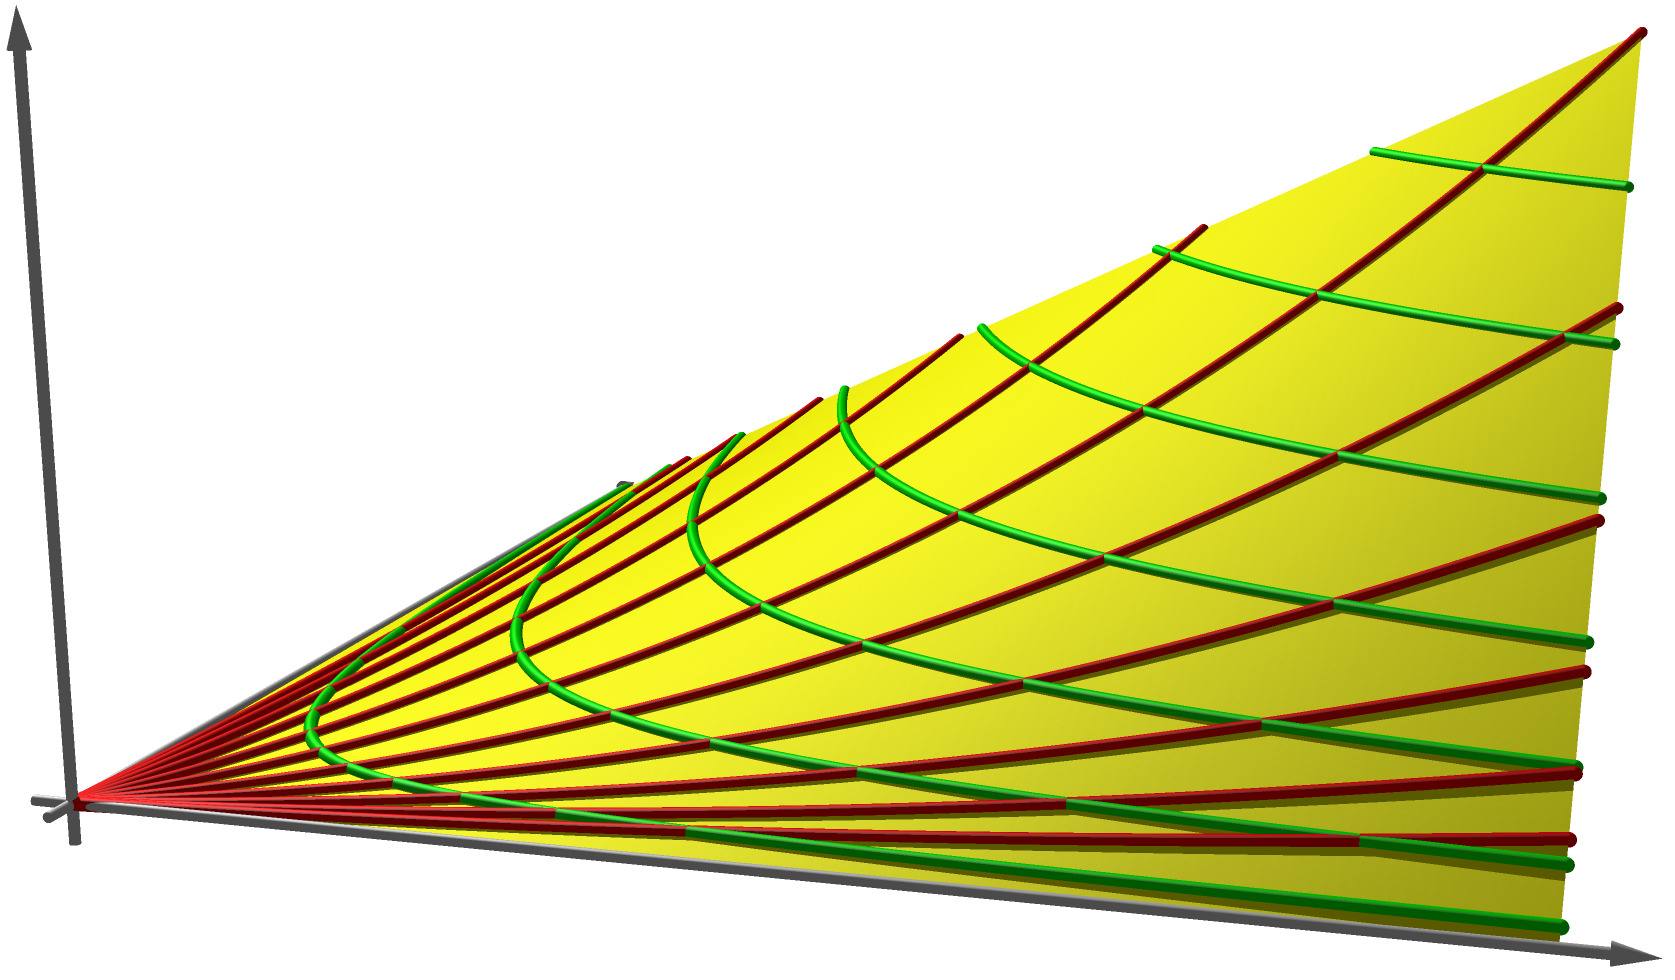
\includegraphics[width=\hsize]{surface.jpg}
\end{center}
\end{frame}


\begin{frame}
\frametitle{Parameterwahl}
Nat"urliche Wahl f"ur ersten Parameter: Kurvenparameter der Cauchy-Anfangskurve
\end{frame}

\begin{frame}
\frametitle{Quasilineare PDGL 1.~Ordnung}
{\bf Differentialgleichung:}
\[
a(x,y,u)\frac{\partial u}{\partial x}+b(x,y,u)\frac{\partial u}{\partial y}
=c(x,y,u)
\]
\pause
Linear, falls $u$ in $a$ und $b$ nicht vorkommen und nur linear in $c$.
\pause

\medskip

{\bf Anfangskurve:}
\pause
\[
u(x_0(t),y_0(t))=u_0(t)
\]
\pause

\smallskip

{\bf Gebiet:} \pause passt!
\end{frame}

\begin{frame}
\frametitle{Normale}
Normale auf Graph von $u(x,y)$:
\pause
\[
\vec n=\begin{pmatrix}
\frac{\partial u}{\partial x}\\
\frac{\partial u}{\partial y}\\
-1
\end{pmatrix}
\]
\pause
Differentialgleichung:
\begin{align*}
0
&=
a(x,y,u)\frac{\partial u}{\partial x}
+
b(x,y,u)\frac{\partial u}{\partial y}
-
c(x,y,u)
\\
&=
{\color{red}
\underbrace{
\begin{pmatrix}
a(x,y,u)\\
b(x,y,u)\\
c(x,y,u)
\end{pmatrix}
}_{\vec t}
}
\cdot
{\color{blue}
\begin{pmatrix}
\frac{\partial u}{\partial x}\\
\frac{\partial u}{\partial y}\\
-1
\end{pmatrix}
}
\end{align*}
\pause
Geometrisch:
\[
{\color{red}\vec t}
\cdot
{\color{blue}\vec n}
=0
\qquad
\Leftrightarrow
\qquad
{\color{red}\vec t}
\perp
{\color{blue}\vec n}
\]

\end{frame}

\begin{frame}
\begin{center}
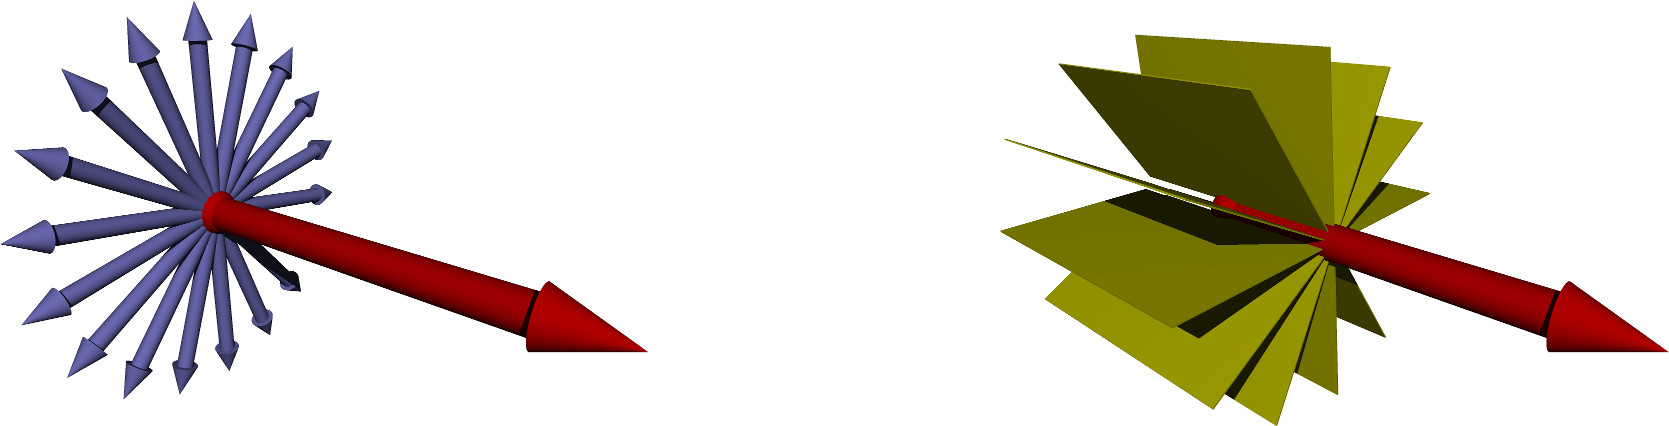
\includegraphics[width=\hsize]{../../skript/3d/normals.jpg}
\end{center}
\end{frame}

\begin{frame}
\frametitle{Charakteristiken}
$
{\color{red}\vec t}
\perp
{\color{blue}\vec n}
$
\pause
$\quad\Rightarrow\quad
\color{red}\vec t$
ist tangential an den Graphen von $u(x,y)$

\bigskip
\pause
Eine Kurve, die $\color{red}\vec t$ als Tangentialvektor hat, 
liegt in der Fl"ache $u(x,y)$

\bigskip
\pause
L"osungsfl"ache wird von {\color{red} Charakteristiken} "uberdeckt

\end{frame}

\begin{frame}
\begin{center}
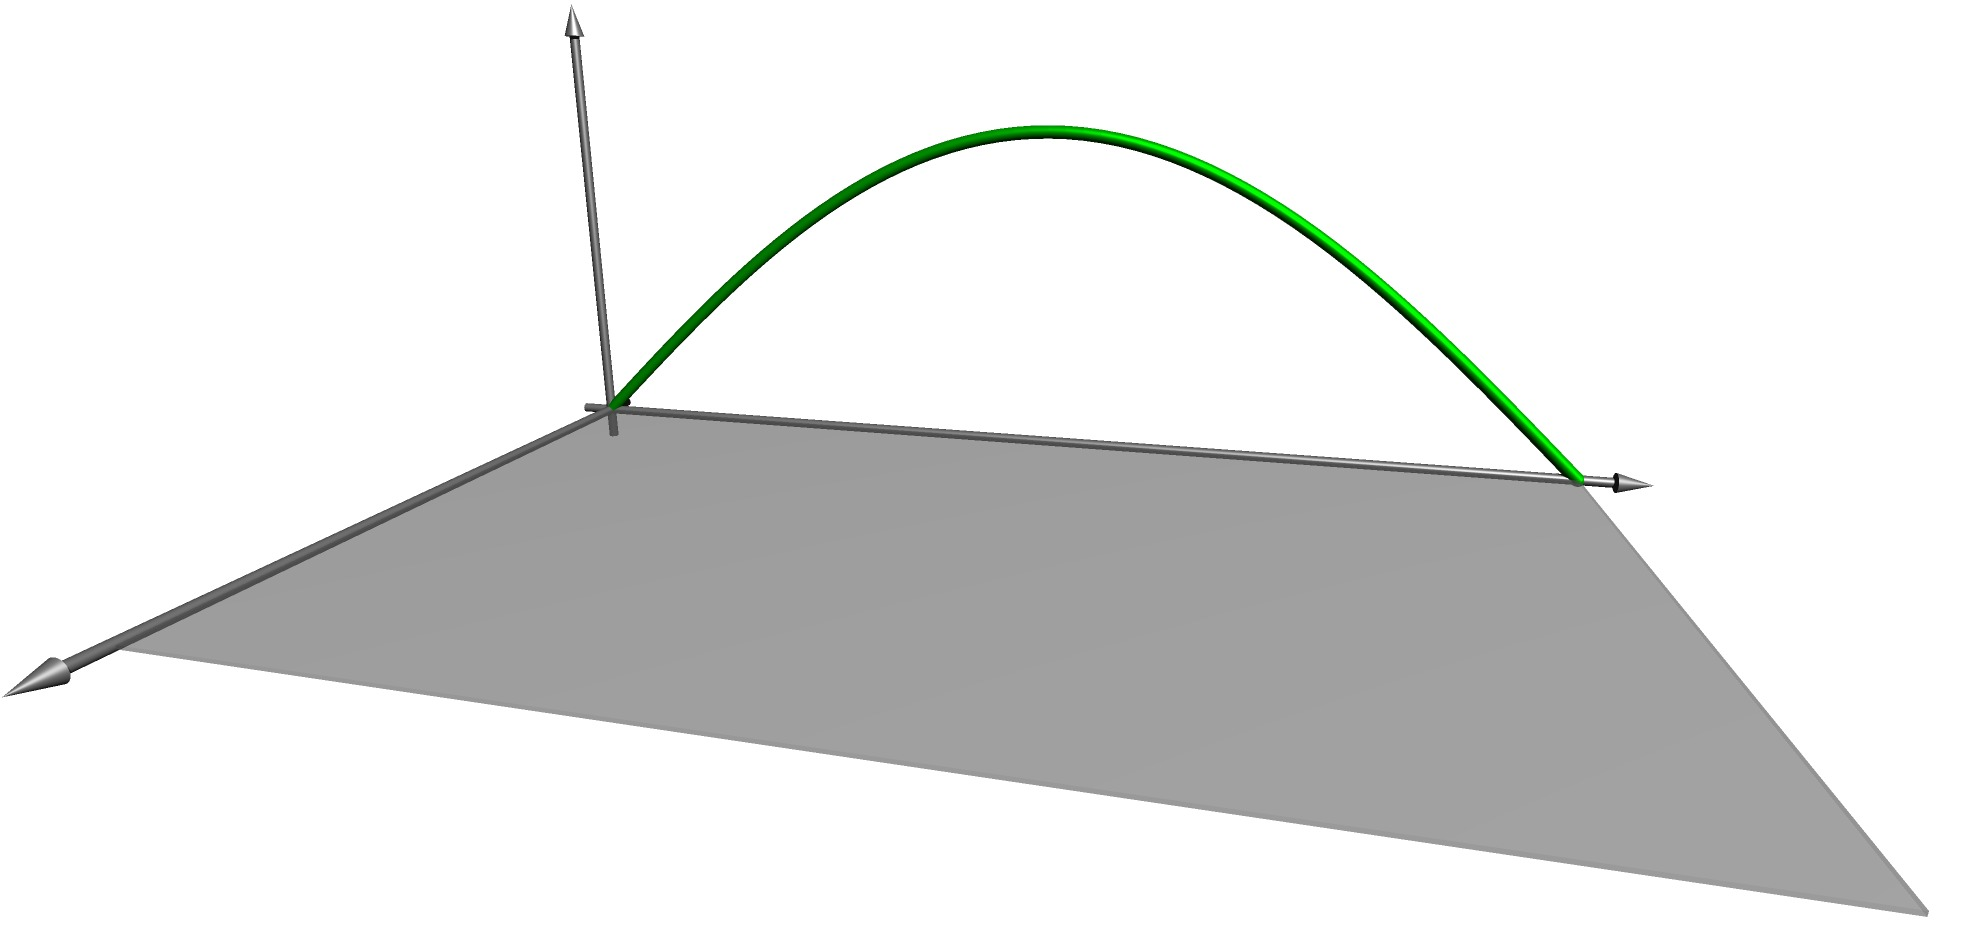
\includegraphics[width=\hsize]{../../skript/3d/cauchy.jpg}
\end{center}
\end{frame}

\begin{frame}
\begin{center}
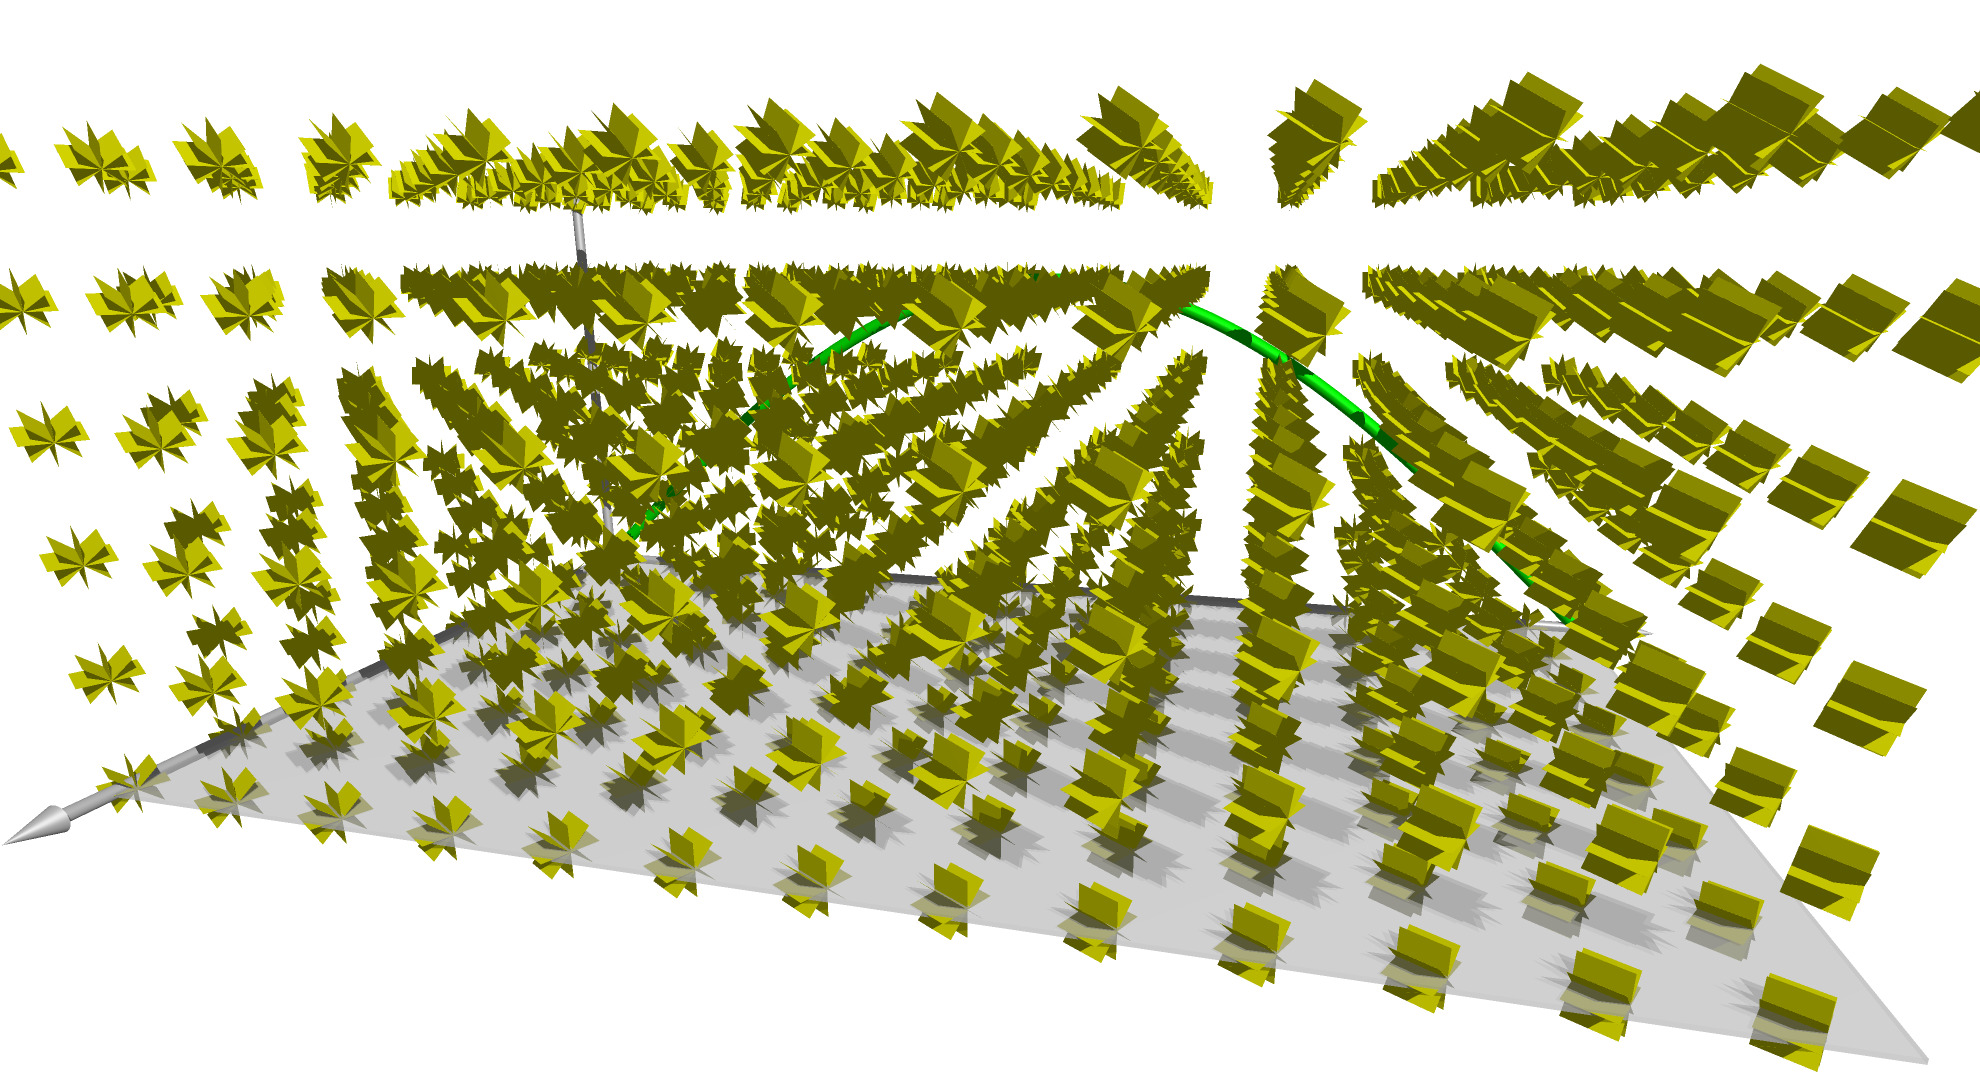
\includegraphics[width=\hsize]{../../skript/3d/planes.jpg}
\end{center}
\end{frame}

\begin{frame}
\begin{center}
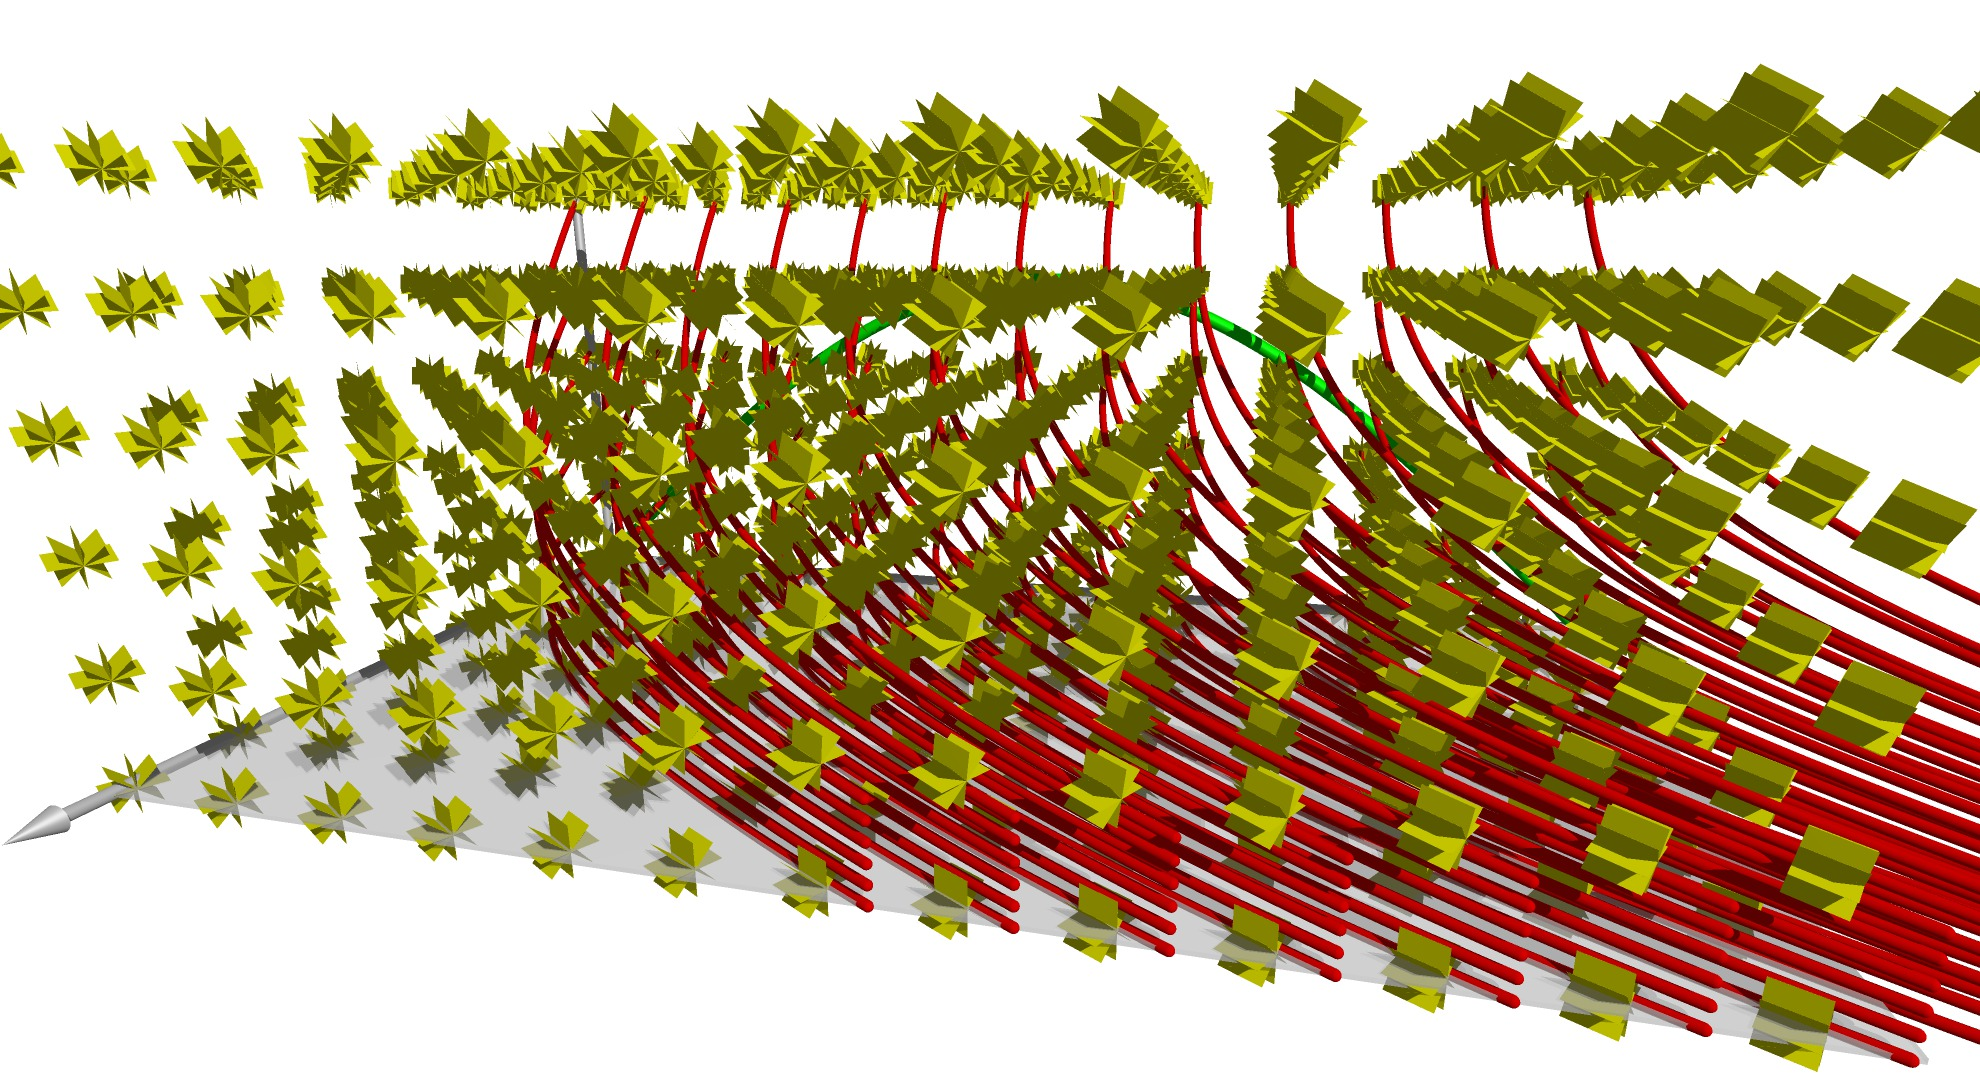
\includegraphics[width=\hsize]{../../skript/3d/chrpl.jpg}
\end{center}
\end{frame}

\begin{frame}
\begin{center}
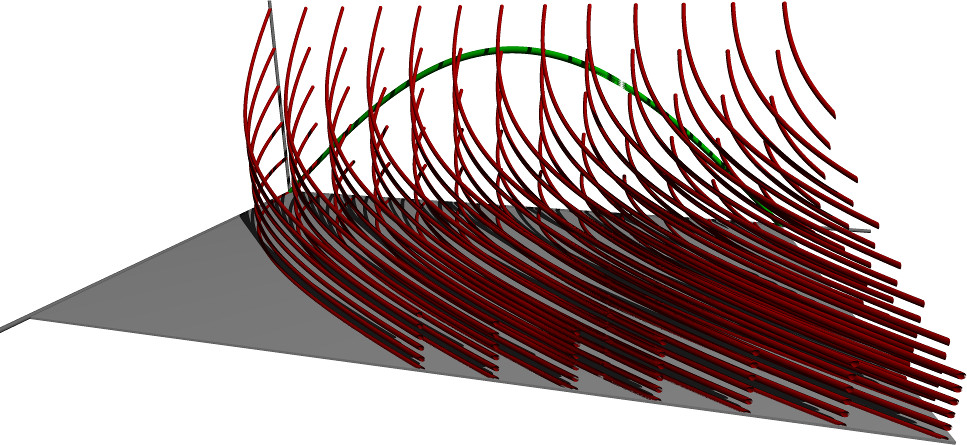
\includegraphics[width=\hsize]{../../skript/3d/chr.jpg}
\end{center}
\end{frame}

\begin{frame}
\begin{center}
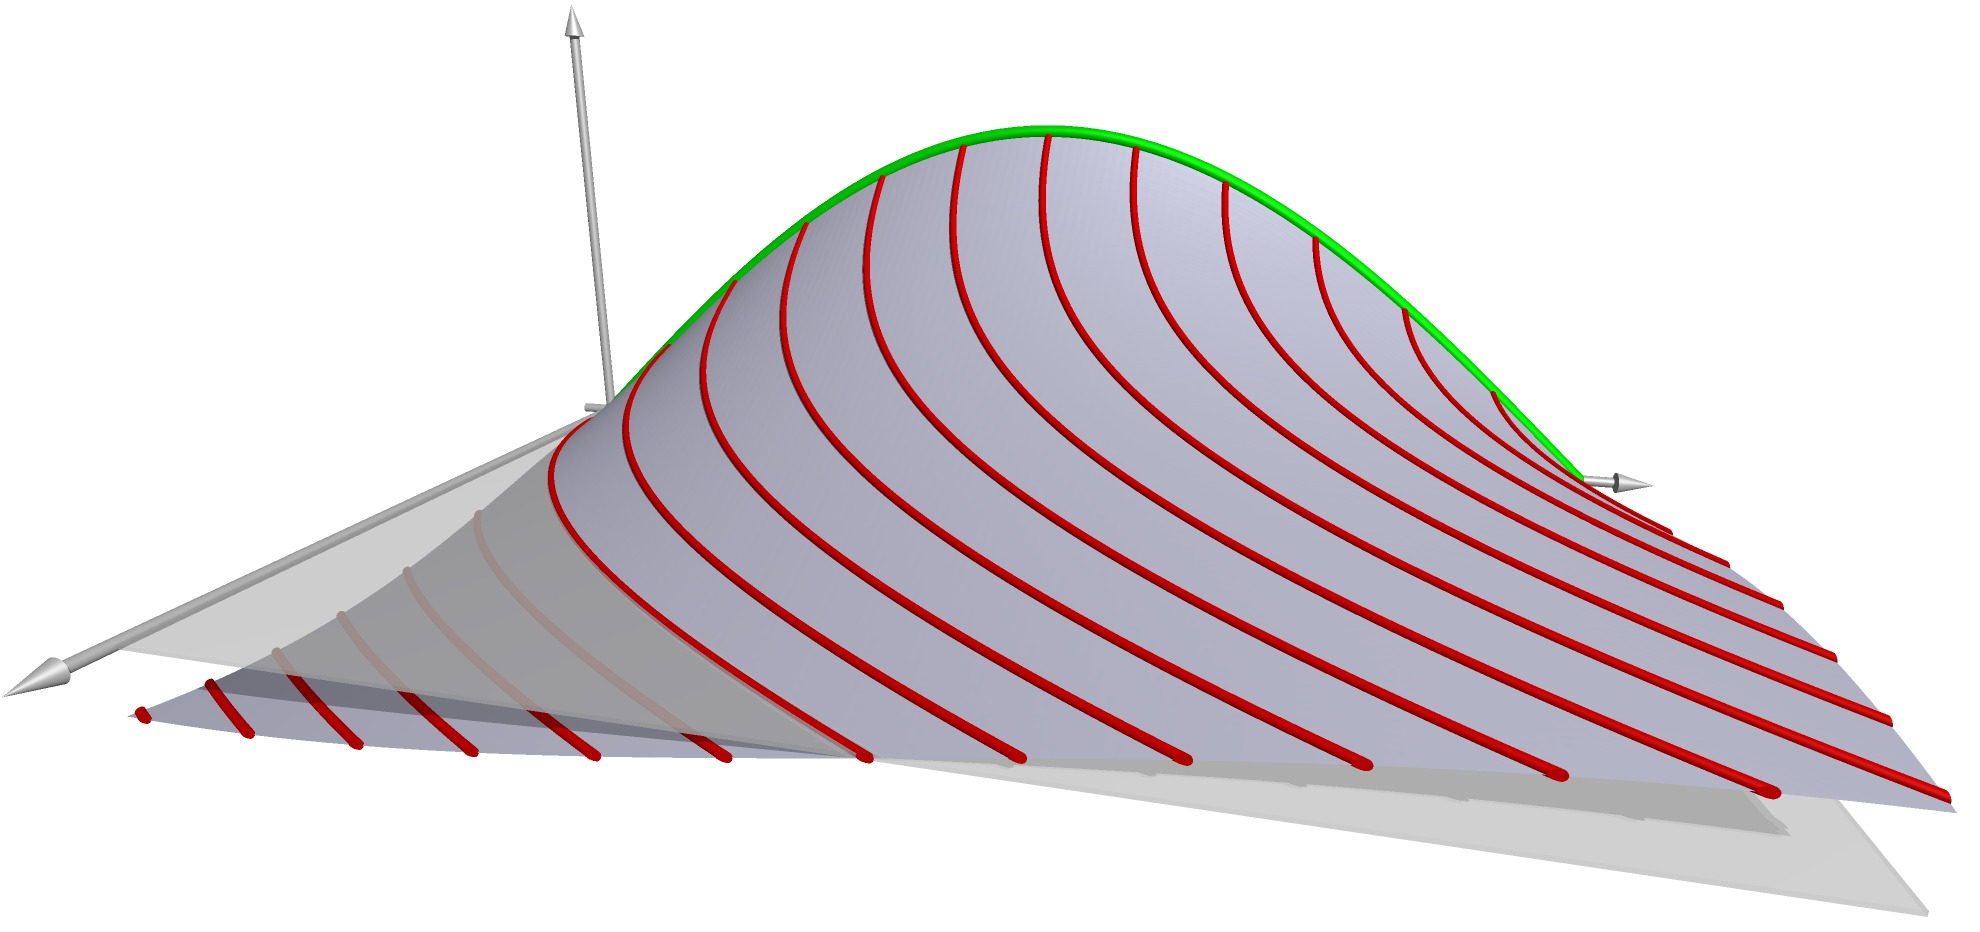
\includegraphics[width=\hsize]{../../skript/3d/sol.jpg}
\end{center}
\end{frame}

\begin{frame}
\frametitle{L"osungsalgorithmus}
\begin{enumerate}
\item Differentialgleichungen f"ur Charakteristiken:
\pause
\begin{align*}
x'(s)&=a(x(s),y(s),u(s))\\
y'(s)&=b(x(s),y(s),u(s))\\
z'(s)&=c(x(s),y(s),u(s))
\end{align*}
\pause
\item Anfangsbedingungen:
\pause
\begin{align*}
x(0)&=x_0(t),&
y(0)&=y_0(t),&
z(0)&=z_0(t)
\end{align*}%
\pause
\item F"ur jedes $t$ eine L"osungskurve $\to$ Eine Fl"ache
\pause
\[
(s,t)\mapsto\begin{pmatrix}
x(s,t)\\
y(s,t)\\
z(s,t)
\end{pmatrix}
\]
\pause
\item L"osung $z=u(x,y)$:
\pause
$s$ und $t$ aus $x$, $y$ und $z$ eliminieren
\end{enumerate}
\end{frame}

\begin{frame}
\frametitle{Beispiel}
{\bf Differentialgleichung:}
\[
\frac{\partial u}{\partial x}
+2
\frac{\partial u}{\partial y}
=3
\]
{\bf Anfangskurve/Randbedingung:}
\[
u(0,y)=\sin y
\]
\begin{enumerate}
\item Differentialgleichung der Charakteristiken
\item Anfangswerte
\item Charakteristiken
\item L"osungsfl"ache
\end{enumerate}
\end{frame}

\begin{frame}
\frametitle{Nichtlinear: Singularit"aten}
Gleichung von Burgers
\[
\frac{\partial u}{\partial t}+u\frac{\partial u}{\partial x}=0
\]
Transportgleichung, Erhaltungssatz

\bigskip
\pause
$\Rightarrow$
Charakteristiken sind Geraden
\end{frame}

\begin{frame}
\frametitle{Nichtlinear: Singularit"aten}
\begin{center}
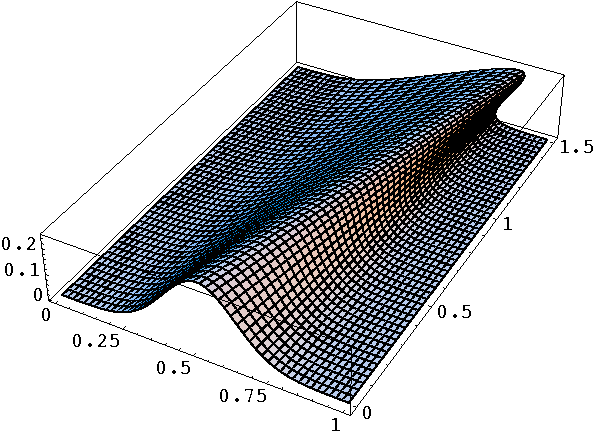
\includegraphics[width=\hsize]{../../skript/graphics/welle.pdf}
\end{center}
\end{frame}

\begin{frame}
\frametitle{Nichtlinear: Singularit"aten}
\begin{center}
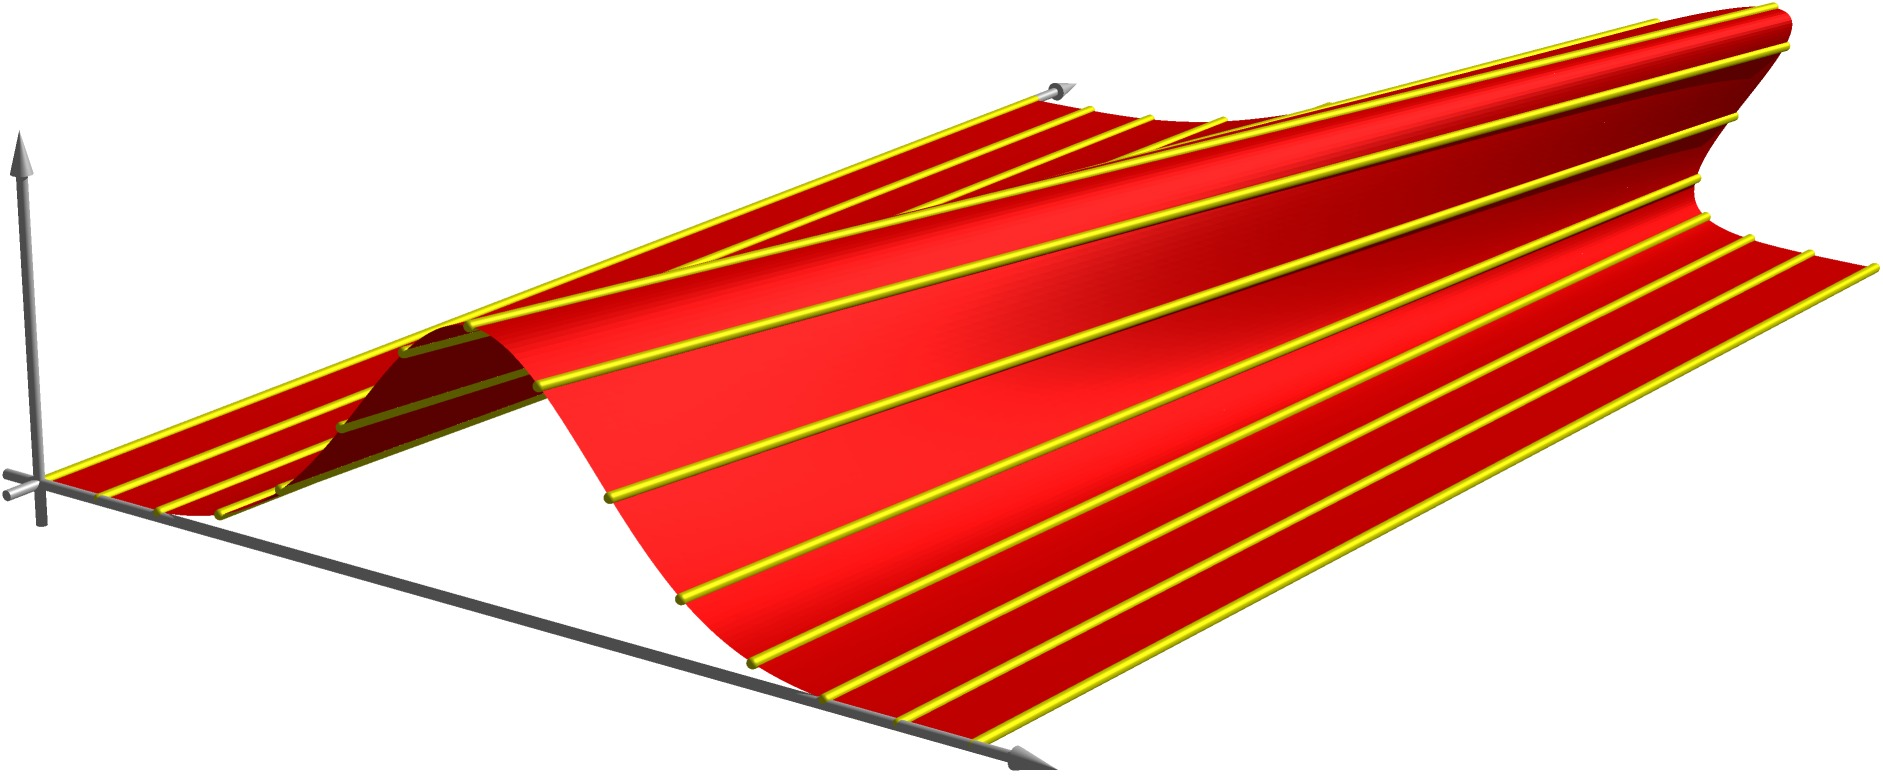
\includegraphics[width=\hsize]{../../skript/graphics/welle.jpg}
\end{center}
\end{frame}

\begin{frame}
\frametitle{Randwerte und Charakteristiken}

{\bf Differentialgleichung:}
\[
\frac{\partial u}{\partial x}
+
2\frac{\partial u}{\partial x}
= 3
\]
{\bf Gebiet:}
\[
\Omega = (0,1)\times(0,1)
\]
\end{frame}

\begin{frame}
\frametitle{Randwerte und Charakteristiken}
\begin{center}
\includegraphics[width=0.6\hsize]{../../skript/images/randwerte-2.pdf}
\end{center}
\end{frame}

\begin{frame}
\frametitle{Randwerte und Charakteristiken}
\begin{center}
\includegraphics[width=0.6\hsize]{../../skript/images/randwerte-3.pdf}
\end{center}
\end{frame}

\begin{frame}
\frametitle{Randwerte und Charakteristiken}
\begin{center}
\includegraphics[width=0.6\hsize]{../../skript/images/randwerte-4.pdf}
\end{center}
\end{frame}

\end{document}
